\section{From Diagnosis to Design: A Two-Axis Verification-Guided Reward}
\label{sec:reward}

Section~\ref{sec:results} established the diagnosis: for frontier models the correctness
signal is \emph{saturated} (the differential verifier changes no outcome) and, by
construction, \emph{gameable} (a serial program earns a perfect score). Because that
same signal is what an agent accepts on and what a verifiable-reward RL loop optimizes
\cite{rlvr,grpo}, the design question follows directly---\emph{what should the reward
measure instead?} This section turns the diagnosis into a design. We define a two-axis
verification-guided reward, then evaluate it in three settings of increasing commitment:
a selection analysis on the study's own accepted programs (Section~\ref{sec:rewardsel});
a best-of-$N$ experiment with live models that stands in for group-relative RL
(Section~\ref{sec:bon}); a two-gate agentic pipeline that repairs correctness and then
scaling (Section~\ref{sec:vgagent}); and GRPO post-training under each reward
(Section~\ref{sec:grpo}). The first is complete and reported here; the others are the
live experiments the released harness runs.

\subsection{The Reward}
\label{sec:rewarddef}
For a generated program $G$ with differential verdict $v$ and measured 8-thread
self-speedup $\mathcal{P}_8$, we compare two rewards. The \emph{correctness-only}
reward---the standard verifiable reward---is
$R_{\text{corr}}(G)=\mathbb{1}[v{=}\textsc{robust}]$, which is $1$ for \emph{every}
robustly-correct program, a serial one included. The \emph{two-axis} reward gates
performance behind correctness,
\begin{equation}\label{eq:twoaxis}
R_{2}(G) \;=\; \mathbb{1}[v{=}\textsc{robust}]\cdot E_8(G),\qquad
E_8(G)=\min\!\big(\mathcal{P}_8(G)/8,\,1\big),
\end{equation}
so a wrong program scores $0$, a correct-but-serial program scores near the floor
$1/8$, and a correct-and-scaling program scores near $1$. A dense, shaped variant used
for RL training awards partial credit toward correctness and then rises with $E_8$
(harness \texttt{rewards.py}). The design point is that $R_2$ is \emph{not} maximized by
serial code, whereas $R_{\text{corr}}$ is.

\subsection{Reward Selection: The Speedup a Correctness Reward Discards}
\label{sec:rewardsel}
The sharpest way to see the cost of the gameable reward needs no new runs. Treat the set
of accepted (robustly-correct) programs for a task as the candidates a
generator---or a best-of-$N$/RL selection---chooses among, and ask which program each
reward selects. $R_{\text{corr}}$ is \emph{indifferent}: every accepted program ties at
$1$, so an uninformed selection realizes, in expectation, the pool's \emph{mean}
speedup. $R_2$ selects the pool \emph{maximum}. On the \NmultiTask{} tasks with more than
one accepted program, the correctness-only reward realizes a mean \RewardRandom{}$\times$
8-thread speedup against the two-axis reward's \RewardTwoAxis{}$\times$
(\RewardGainPct{}\% higher; Fig.~\ref{fig:reward}). The gap is starkest within a single
task: on \RewardSpreadTask{} the accepted programs run from \RewardSpreadLo{}$\times$ to
\RewardSpreadHi{}$\times$, all rated identically by $R_{\text{corr}}$. A correctness-only
objective is not merely blind to this spread---it discards it.

\begin{figure}[t]
\centering
\IfFileExists{../results/figures/fig_reward_selection.pdf}
  {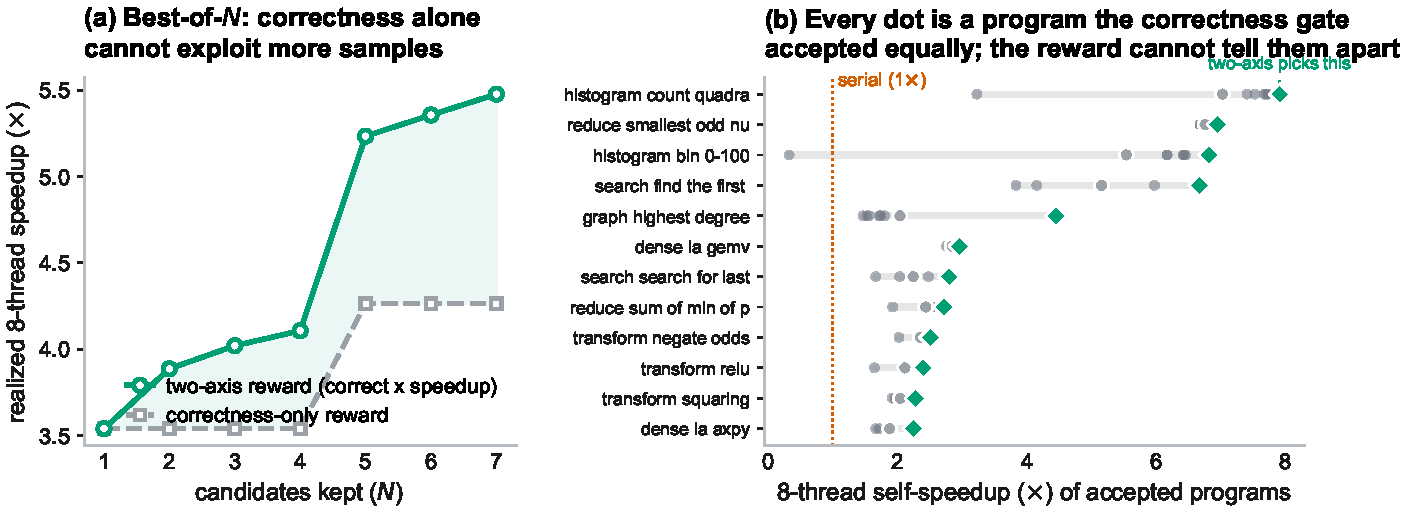
\includegraphics[width=\linewidth]{../results/figures/fig_reward_selection.pdf}}
  {\fbox{\parbox{0.9\linewidth}{\centering\vspace{2em}\textsc{[reward-selection figure]}\vspace{2em}}}}
\caption{The speedup a correctness-only reward leaves on the table. \textbf{(a)}~As more
candidates are kept ($N$), the two-axis reward realizes a rising fraction of the
available speedup while the correctness-only reward stays flat at the pool mean---it has
no signal to exploit additional samples. \textbf{(b)}~Every dot is a program the
correctness gate accepted equally; a correctness-only reward cannot prefer the fast ones
(diamonds) over the slow ones. Data: the \Ntimed{} accepted programs of
Section~\ref{sec:scaling}.}
\label{fig:reward}
\end{figure}

\subsection{Best-of-$N$ with Live Models}
\label{sec:bon}
Reward selection above reuses the frozen study; here we reproduce the effect with fresh
sampling, as a faithful and inexpensive proxy for what group-relative RL (GRPO) would
learn---GRPO scores a group of samples with a verifiable reward and moves toward the
higher-scoring ones, and best-of-$N$ is that selection without the gradient step. For
each of \xx{} race-prone tasks and \Nmodels{} models we draw $N{=}\xx{}$ single-shot
completions, verify each with the differential gate, time the correct ones, and select
under each reward. The correctness-only reward realizes a mean \xx$\times$ 8-thread
speedup (a random correct pick); the two-axis reward realizes \xx$\times$ (\xx\% higher),
and in \xx{} of \xx{} pools the two rewards select \emph{different} programs
(Table~\ref{tab:bon}). Because the two rewards are computed over the \emph{same} samples,
the difference is attributable entirely to the reward, not to the model or the decoding.

\begin{table}[t]
\caption{Best-of-$N$ ($N{=}\xx$) reward selection with live models on the race-prone
task subset. Realized 8-thread self-speedup under each reward; the correctness-only
reward selects a random correct program, the two-axis reward the fastest.}
\label{tab:bon}
\centering\footnotesize
\begin{tabular}{@{}lccc@{}}
\toprule
Model & corr.-only ($\times$) & two-axis ($\times$) & pools differing \\
\midrule
\xx & \xx & \xx & \xx \\
\xx & \xx & \xx & \xx \\
\xx & \xx & \xx & \xx \\
\midrule
mean & \xx & \xx & \xx \\
\bottomrule
\end{tabular}
\end{table}

\subsection{VG-RLPT: A Two-Gate Agentic Pipeline}
\label{sec:vgagent}
The reward suggests a controller. We instantiate it as a verification-guided agent that
decomposes generation into two temporally-abstracted options with execution-based
termination (Sec.~\ref{sec:rewarddef}; Fig.~\ref{fig:vgpipeline}). In
$\omega_{\text{correct}}$ a tool-using coder agent writes the function and invokes the
differential verifier itself, repairing until the verdict is \textsc{robust}
($\beta_{\text{correct}}$). Control then passes to $\omega_{\text{parallel}}$, in which
an optimizer agent invokes a timing tool, diagnoses the bottleneck, and rewrites for
speed---re-verifying correctness after every change, so the performance gate is
\emph{guarded}: an optimization that breaks correctness is rejected and the last robust
program is restored ($\beta_{\text{parallel}}$ fires only when the program both scales
and remains robust). The agents drive their own tool calls; the meta-policy is a state
machine over the two options (harness \texttt{agentic/}).

Against the correctness-only baseline (Section~\ref{sec:ablation}, which stops at
$\omega_{\text{correct}}$), the pipeline lifts \xx{} of \xx{} accepted-but-slow programs
past the scaling target, raising mean 8-thread self-speedup from \xx$\times$ to
\xx$\times$ at unchanged robust correctness (\xx\%). The canonical case is the histogram
of Section~\ref{sec:crosscap}: the correctness-only agent ships a robust but
critical-serialized version at \xx$\times$; the two-gate agent, seeing the timing tool's
verdict, rewrites it to a per-thread reduction at \xx$\times$, still robust. Full
per-run tool traces are released.

\begin{figure}[t]
\centering
\IfFileExists{../results/figures/fig_vg_pipeline.pdf}
  {\includegraphics[width=\linewidth]{../results/figures/fig_vg_pipeline.pdf}}
  {\fbox{\parbox{0.9\linewidth}{\centering\vspace{1.5em}\textsc{[VG-RLPT two-gate
   pipeline schematic: $\omega_{\text{correct}}\!\to\!\omega_{\text{parallel}}$, each
   gated by a verifier]}\vspace{1.5em}}}}
\caption{The VG-RLPT pipeline. The coder option terminates when the differential
verifier certifies correctness; the optimizer option, guarded by re-verification,
terminates when the program clears a speedup target while staying robust. Only the
performance gate is new; the correctness gate is the study's differential verifier.}
\label{fig:vgpipeline}
\end{figure}

\subsection{GRPO Post-Training on the Two-Axis Reward}
\label{sec:grpo}
Finally we test the prediction as a training outcome: a model post-trained with GRPO on
the correctness-only reward should drift toward ``correct but not parallel'', while the
same procedure on the two-axis reward should not. We post-train \xx{} (e.g.\
\texttt{Qwen2.5-Coder-\xx B}) with GRPO under each reward, computing the verifiable
reward by compiling and timing every sampled completion against ParEval's reference. The
two arms reach comparable robust correctness (\xx\% vs.\ \xx\%), but their sampled
8-thread self-speedup diverges over training (Fig.~\ref{fig:grpo}): the correctness-only
arm is flat/declining at \xx$\times$, the two-axis arm rises to \xx$\times$. Optimizing
the gameable reward buys correctness at the cost of the parallelism; optimizing the
two-axis reward keeps both.

\begin{figure}[t]
\centering
\IfFileExists{../results/figures/fig_grpo.pdf}
  {\includegraphics[width=\linewidth]{../results/figures/fig_grpo.pdf}}
  {\fbox{\parbox{0.9\linewidth}{\centering\vspace{1.5em}\textsc{[GRPO training curve:
   sampled 8-thread self-speedup vs.\ step, two reward arms]}\vspace{1.5em}}}}
\caption{GRPO post-training under each reward. Mean 8-thread self-speedup of the policy's
sampled programs versus training step: the correctness-only reward (\xx) does not improve
parallelism; the two-axis reward (\xx) does, at equal correctness.}
\label{fig:grpo}
\end{figure}
